\documentclass[12pt,a4paper]{article}
\usepackage[utf8]{inputenc}
\usepackage[english]{babel}
\usepackage[T1]{fontenc}
\usepackage{amsmath}
\usepackage{amsfonts}
\usepackage{amssymb}
\usepackage{subcaption}
\usepackage{makeidx}
\usepackage{graphicx}
\usepackage{fourier}
\usepackage{listings}
\usepackage{color}
\usepackage{hyperref}
\usepackage[left=2cm,right=2cm,top=2cm,bottom=2cm]{geometry}
\author{Tommy Müller, Marcus Dittrich, Vincent Noculak}
\title{Holographie}


\lstset{language=C++,
	keywordstyle=\bfseries\color{blue},
	commentstyle=\itshape\color{red},
	stringstyle=\color{green},
	identifierstyle=\bfseries,
	frame=single}
\begin{document}

\maketitle
\newpage
\tableofcontents
\newpage
	
\section{Theorie}

\subsection{Einleitung}

Die Holographie ist ein von Dennis Gabor entwickeltes Verfahren zur räumlichen Abbildung von Objekten. Im Gegensatz zur herkömmlichen Photographie, welche nur Informationen über die Intensität des Lichtwellenfeldes eines abgebildeten Gegenstandes aufnimmt, ermöglicht Holographie die Darstellung räumlicher Charakteristika. Dafür werden Phase und Amplitude durch Hinzunahme einer Referenzwelle gespeichert.Grundbedingung hierfür ist die Kohärenz des Lichtes um eine feste Phasenbeziehung zwischen Objekt und Referenzwelle zu erhalten. Die Phasenbeziehung ist dann aus dem entstehenden Interferenzmuster auf der Photoplatte, zwischen Objekt- und Referenzwelle, abzulesen. Das erhaltene Bild hat zunächst keine Ähnlichkeit mit dem Orginalobjekt, es muss erst wieder speziell beleuchtet werden um ein dreidimensionales Abbild des Objektes zu erhalten. Da Objekt- und Referenzwelle die gleiche Wellenlänge besitzen, dürfen die Bauteile des Versuchsaufbaus innerhalb der Belichtungsdauer nur um einen Bruchteil ihrer Wellenlänge ($\lambda/4$) bewegt werden, um das Interferenzmuster nicht zu verzerren. Da meist ein HeNe-Laser mit einer Wellenlänge von $\lambda = 632nm$ verwendet wird, reichen leichte Erschütterungen aus, um das entstehende Bild unbrauchbar zu machen. Deswegen benötigen wir ein Instrument, um unseren Aufbau auf die nötige Stabilität zu Prüfen. 

\subsection{Michelson-Interferometer}

In unserem Aufbau wir dafür ein Michelson-Interferometer benutzt. Im Allgemeinen besteht die Funktionsweise eines Interferometers darin, eine einfallende Lichtwelle in zwei Wellen zu teilen. Diese durchlaufen dann unterschiedlich lange Wegstrecken, wodurch sich eine Phasenverschiebung zwischen beiden Wellen ergibt. Werden beide Wellen wieder zusammengefügt, kommt es zur Interferenz. \begin{figure}[h]
	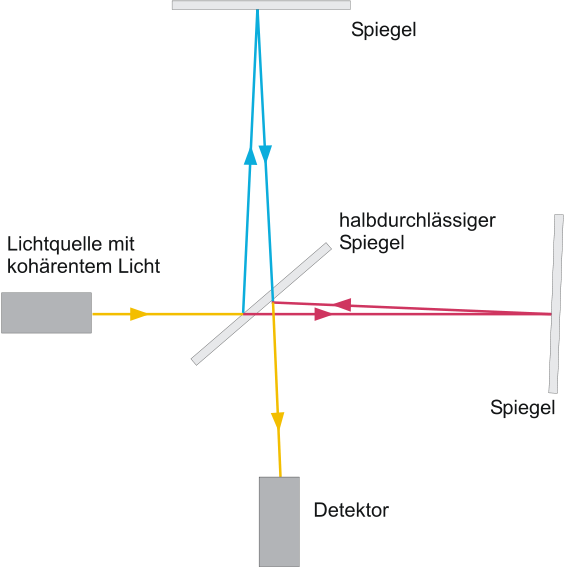
\includegraphics[scale = 0.5]{Michelson.png}
	\centering
	\caption{Schematischer Aufbau eines Michelson-Interferometers}
	\label{11}
\end{figure}Im Michelson-Interferometer wird der einfallende Strahl aus einer koherenten Lichtquelle im Zentrum des Aufbaus durch einen halbdurchlässigen Spiegel geteilt. Anschließen werden die beiden Strahlen reflektiert und im Zentrum wieder zusammengefügt und auf dem Detektor zur Interferenz gebracht. Ist auf dem Detektor ein Interferenzmuster zu erkennen, so ist der Weglängenunterschied den beide Wellen durchlaufen haben innerhalb der Kohärenzlänge der Strahlungsquelle. Minimale Veränderungen der Weglänge sind anhand von Änderungen des Interferenzmusters auf dem Detektor zu erkennen. Somit kann über die Beobachtung der Interferenzmuster die Stabilität des Aufbaus abgeschätzt werden. Der schematische Aufbau des Michelson-Interferometers wird in Figure $\ref{11}$ dargestellt.

\subsection{Physikalische Grundlagen}

\subsubsection{Kohärenz}

Als Kohärenz wird die Eigenschaft einer Lichtquelle bezeichnet, mit sich selber interferieren zu können. Bedingung dafür ist, das die Lichtquelle monochromatisch ist und eine feste Phasenbeziehung zwischen den einzelnen Teilwellen besteht.

\subsubsection{Interferenz und Beugung}

Als Interferenz bezeichnet man die Überlagerung zweier kohärenter Wellen. Dabei gibt es zwei Extremfälle, die konstruktive und die destruktive Interferenz. Bei der konstruktiven Interferenz liegen Minima und Maxima übereinander, wodurch die Amplituden addiert werden. Bei destruktiver Interferenz sind die beiden Wellen um $/pi /2$ zueinander verschoben, wodurch sich die Wellenfunktionen bei gleicher Amplitude auslöschen. Schickt man einen kohärenten Lichtstrahl durch ein optisches Gitter, dessen Gitterkonstante in etwa der Wellenlänge des einfallenden Lichts entspricht, so ergibt sich auf dem Schirm hinter dem Gitter ein Interferenzmuster. Diese Muster entstehen durch Interferenz der, am Gitter neu entstehenden Wellen, miteinander. Des Weiteren gibt es Beugung am Kristallgitter, bei dem Interferenz durch Reflexion an den regelmäßig angeordneten Kristallgittern entsteht. Dafür lässt sich die Bragg-Bedingung festhalten, welche für die Reflexionsholographie von Bedeutung sein wird:

\begin{equation}
2k \frac{\lambda}{2} = |2d sin \nu|
\label {1}
\end{equation}
	
\subsection{Varianten der Holographie}

Es gibt mehrere Möglichkeiten Holographie zu betreiben, welche sich Grundlegend durch ihren Aufbau unterscheiden. Zwei der wichtigsten sind die Transmissions- und die Reflexionsholographie, welche wir in den folgenden Absätzen näher erläutern wollen. 

\subsubsection{Transmissionsholographie}

\begin{figure}[h]
	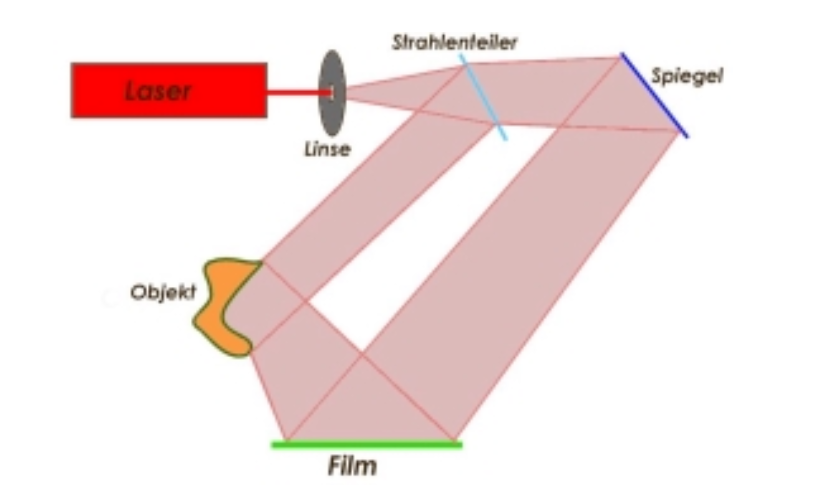
\includegraphics[scale = 0.5]{Trans.png}
	\centering
	\caption{Möglicher Aufbau zur Aufnahme eines Transmissionshologramms}
	\label{22}
\end{figure}

In Figure $\ref{22}$ wird eine Möglichkeit des schematischen Aufbaus zur Transmissionsholographie dargestellt. Eine kohärente Lichtquelle emittiert  Licht, welches in einem halb durchlässigen Spiegel geteilt wird. Der eine Strahl trifft auf das zu untersuchende Objekt, von welchem es auf die Photoplatte reflektiert wird. Der sog. Referenzstrahl wird hinter dem Strahlenteiler unverändert auf die Platte geleitet. Um den Vorgang theoretisch zu beschreiben muss man Objekt- und Referenzwelle überlagern und aus der Summe der Amplituden die Intensität bestimmen. An einem Ort (x,y) auf der Photoplatte ergibt sich für die elektrische Feldstärke:
\begin{equation}
\ E(x,y,t) = O(x,y,t) + R(x,y,t)
\label {1}
\end{equation}
geht man davon aus, das für $O(x,y,t)=O(x,y)*e^{-i\omega t}$ und $R(x,y,t)=R(x,y)*e^{-i\omega t}$ gilt, so ergibt sich für die Intensität:

\begin{equation}
\ I(x,y) = |O(x,y) + R(x,y)|^{2} = (O+R)(O+R)^{*} = RR^{*} + OO^{*} + R^{*}O + O^{*}R
\label {1}
\end{equation}
Bei $R^{*}$ und $ O^{*}$ handelt es sich um komplex konjugierte Amplituden. Während der kompletten Belichtungszeit reagiert die Photoplatte auf die einfallende Energie pro Fläche und setzt dies in eine Schwärzung der Photoplatte mit Veränderung des Brechungsindexes am Ort (x,y) um. Die Belichtung B [Energie/Fläche] ist über folgendes Integral bestimmt, wobei $t_{b}$ die Belichtungszeit ist:
\begin{equation}
\ B(x,y) = \int_{0}^{t_{b}}I(x,y) 
\label {1}
\end{equation}
Die Belichtung führt zu einer komplexen Amplitudentransmission des Negativs. Dafür lässt sich der komplexe Amplitudentransmissionsgrad $\tau$ bestimmen:
\begin{equation}
\tau = \frac{E_{a}}{E_e}  = Te^{i\psi} = |\tau|e^{i\psi}
\label {1}
\end{equation}
$E_{a}$ und $E_{e}$ sind hierbei die einfallende und die auslaufende Welle. Für den komplexen Amplitudentrainsmissionsgrad gilt als Funktion des Ortes auf der Photoplatte:
\begin{equation}
\tau = \frac{E_{a}}{E_e} = \tau(x,y) = T(x,y)e^{i\psi(x,y)} 
\label {1}
\end{equation}
Es gibt zwei gängige Arten zur Betrachtung des Problems, bei der einen nimmt man $\psi$ = const an, dem sog. Amplitudenhologramm. Bei der anderen geht man davon aus, das T = const und erhält das sog. Phasenhologramm. Für beide Varianten lässt sich der Verlauf der Amplitude und der Phase in Abhängigkeit von der Belichtung B skizzieren, wie in Figure $\ref{33}$ $\&$ $\ref{44}$ zu sehen ist.
\begin{figure}[h]
	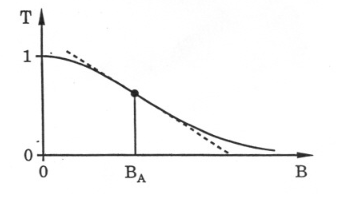
\includegraphics[scale = 0.5]{Amptrans.png}
	\centering
	\caption{Verlauf von T über B beim Amplitudenhologramm}
	\label{33}
\end{figure}
\begin{figure}[h]
	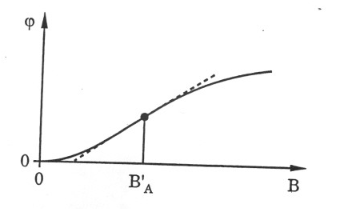
\includegraphics[scale = 0.5]{Phasentrans.png}
	\centering
	\caption{Verlauf von $\psi$ über B beim Phasenhologramm}
	\label{44}
\end{figure}

Beide Funktionen werden um einen Arbeitspunkt $B_{A}$ linear genähert. Für das Amplitudenhologramm gilt somit der Zusammenhang:

\begin{equation}
T = a- bB = a-bIt_{B}
\label {1}
\end{equation}

Für das Phasenhologramm ergibt sich für die lineare Näherung in der Umgebung des Arbeitspunktes $B_{A}$:

\begin{equation}
\psi(I) = a^{'} + b^{'}tIt_{B}
\label {1}
\end{equation}

Dies führt zu:

\begin{equation}
\tau = e^{i\psi(I)} 
\label {1}
\end{equation}

Um dafür den linearen Zusammenhang zu erhalten entwickelt man die Exponentialfunktion für $\psi(I) << \pi/2$ und bricht nach dem linearen Glied ab, so dass man folgenden Zusammenhang erhält:

\begin{equation}
\tau = e^{i\Psi(I)} = 1 + i\Psi(I)
\label {3}
\end{equation}

Sowohl beim Amplitudenhologramm, als auch bei Phasenhologramm gilt der Zusammenhang:

\begin{equation}
\tau(x,y) \propto I(x,y)
\label {2}
\end{equation}

Um die entwickelte Photoplatte auswerten zu können, wird der Laser auf die Platte gerichtet. Ein Teil des Lichts transmittiert durch die Platte entsprechend des Transmissionskoeffizienten $\tau$, welcher  Ortsgebunden proportional zur Intensität bei der Hologrammerzeugung ist, wie in Gleichung $\ref{2}$ beschrieben. Man erhält hinter der Hologrammfläche für das Amplitudenhologramm die komplexe Amplitude $E_{a}$:

\begin{equation}
E_{a}(x,y) = T(x,y)E_{e} = T(x,y)R = Ra-bt_{B}R(RR^{*} + OO^{*} + R^{*}O + O^{*}R)
\label {1}
\end{equation}

Die vier Terme der Gleichung haben der Reihe nach folgende Bedeutungen, die ersten beiden Terme sind die Nullte Ordnung der Referenzwelle, jeweils mit einem konstanten Faktor multipliziert. Der dritte Term ist das virtuelle Bild, welches sowohl Objektamplitude als auch Objektphase enthält, während der vierte Term das konjugierte Bild des Objektes, in unserem Fall eine Störung ist. Um ein möglichst gutes Bild zu erhalten, versucht man die Störterme zu minimieren. Die Rekonstruktion des Bildes mithilfe eines Phasenhologramms ist analog dazu mit dem Transmissionskoeffizienten aus Gleichung $\ref{3}$. Im Vergleich zwischen Phasen- und Amplitudenhologramm liefert das Phasenhologramm das hellere Bild, dafür hat es allerdings mehr Störeffekte. 

\subsubsection{Reflexionsholographie}

Im Gegensatz nur Transmissionsholographie treffen Objekt- und Referenzwelle von unterschiedlichen Seiten auf die Photoplatte. Des Weiteren ist diese anders beschaffen, sie besteht aus einer wesentlich dickeren Gelatineschicht, welche Interferenzbilder in verschiedenen Ebenen aufnehmen kann. Daher spricht man im Falle der Reflexionsholographie auch von Volumenhologrammen, während man Transmissionshologramme auch als Flächenhologramme bezeichnet. In Figure $\ref{55}$ wird eine Möglichkeit des schematischen Aufbaus zur Reflexionsholographie dargestellt. 
\begin{figure}[h]
	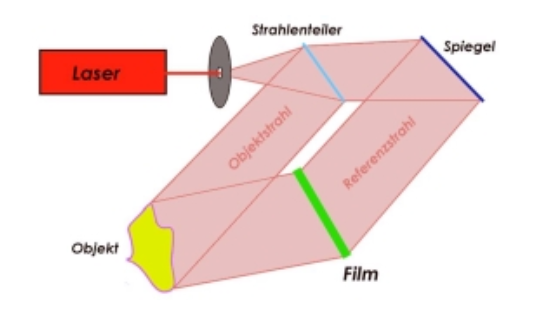
\includegraphics[scale = 0.5]{Refl.png}
	\centering
	\caption{Möglicher Aufbau zur Aufnahme eines Reflexionshologramms}
	\label{55}
\end{figure}
Dabei bilden Objekt- und Referenzstrahl innerhalb des Photomaterials stehende Wellen aus, wodurch in mehreren Ebenen ein Interferenzmuster erzeugt wird, was in Figure $\ref{66}$ schematisch dargestellt ist. Die Skizze veranschaulicht außerdem das entstehen mehrerer Netzebenen innerhalb des Photomaterials. 

\begin{figure}[h]
	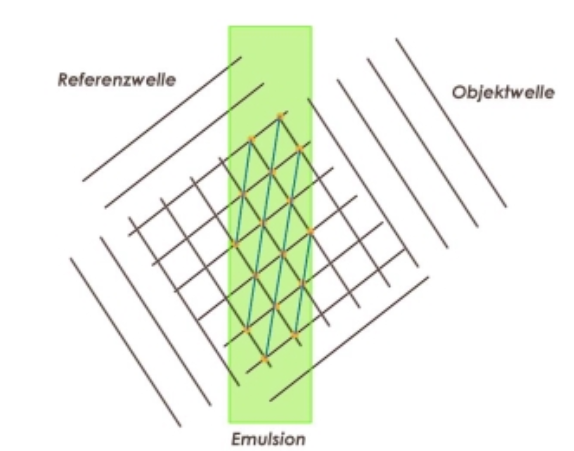
\includegraphics[scale = 0.5]{refsteh.png}
	\centering
	\caption{Entwicklung der Netzebenen innerhalb des Photomaterials}
	\label{66}
\end{figure}

Die verschiedenen Ebenen entsprechen dabei Reflexionsgittern. Der Abstand der Netzebenen zueinander wird durch die Wellenlänge $\lambda$ und Winkel des einfallenden Lichts $\nu$ bestimmt. Es gilt folgender Zusammenhang:

\begin{equation}
d = \frac{1}{2} \frac{\lambda}{|sin \nu|}
\label {1}
\end{equation}

Um das Hologramm darstellen zu können wird die Reflexion des Referenzstrahl durch das Photomaterial geschickt. Der einfallende Lichtstrahl wird an den Netzebenen nach der Bragg-Bedingung reflektiert. Wird der Einstrahlungswinkel $\nu$ variiert ist die Bedingung nicht mehr erfüllt und das Objekt kann nicht wiedergegeben werden. Die Bragg-Bedingung ermöglicht es die Rekonstruktion auch mit "weißem" Licht durchzuführen, da bestimmte Teilwellen die Bedingungen erfüllen. Dabei erhält man Licht verschiedener Wellenlängen, was zu unterschiedlichen Farbgebungen führt. 

\subsubsection{Andere Verfahren}

Reflexions- und Transmissionholograhpie sind die Grundlagen aller holographischen Verfahren. Allerdings gibt es noch einige, welche auf den Grundlagen der zuvor genannten Verfahren beruhen, sich allerdings im Versuchsaufbau unterscheiden. Das vermutlich bekannteste ist Denisjuk-Hologramm, benannt nach dem sowjetischen Physiker Juri Nikolajewitsch Denisjuk. Dabei handelt es sich um eine Vereinfachung der Reflexionsholographie. Hierbei wird der Laserstrahl nicht geteilt. der Strahl wird durch eine Linse aufgeweitet und durchleuchtet als Referenzstrahl das Photomaterial. Das zu untersuchende Objekt befindet sich hinter der Photofläche und wird teilweise als Objektstrahl zurück reflektiert. Dadurch entsteht wieder Interferenz nach dem Verfahren der Reflexionsholographie. Der schematische Aufbau lässt sich in Figure $\ref{77}$ nachvollziehen.

\begin{figure}[h]
	\includegraphics[scale = 0.5]{denis.png}
	\centering
	\caption{Stabilitätsdiagramm einer Paulfalle}
	\label{77}
\end{figure}
\section{Quelle}

Abb2 http://www.holografie.com/Fouquier.pdf




\end{document}